\documentclass[../report.tex]{subfiles}

\begin{document}

\color{red}
\charactercount{introduction} (incl. spaces)
\color{black}
\pagebreak

\section{INTRODUCTION}

As the prevalence of smartphones and internet of things (IoT) devices increasingly dictate the human experience, the software industry has pivoted connectivity-centered development. A common mobile software application is fully reliant on an internet connection, acting almost exclusively as a recipient for transmitted data. These clients typically serve purposes such as social media communication, content consumption, user account access etc.

This reliance on connectivity means the software becomes a front-end client in a distributed computing system, with the logistical and computational responsibilities assigned and distributed to and among a network of back-end servers. With this reality comes a series of architectural considerations and decisions that inform how and to what extent the front-end software is developed. \\

A main feature of distributed systems is their ability to handle hardware and software heterogeneity, as information must travel digitally and physically across layers of applications, networks, and hardware. Another feature is their ability to transmit and parse information across layers despite the differences in protocols, programming language features, and data formats. As data transmission has become ubiquitous, . Section \ref{sec:vocabulary} explores the landscape of distribution and data transmission in-depth, to establish a vocabulary of terminology. \\

Existing research predominantly evaluates data serialisation formats from a feature, performance, and efficiency perspective. While these aspects are quantifiable, measurable, and potentially motivate decisions at large-scale data transmission they fail to illustrate the conditions that inform the choice of data format for the common software development team. These conditions are likely more abstract and extend beyond development into the organisational structures and division of ownership in the team or company. \\

The contribution of this paper is to evaluate the balance between readability and safety in the JSON data serialisation format, in order to propose an extensible format informed by the value perspective of developers. This proposed format, conceptualised as the Type-Extensible Object Notation (TXON), is paired with a translation layer written in JavaScript, to provide full compatibility with JSON data and language parsers.

There exists a rich history of design philosophy in programming language and data format syntax, features, and architecture. It is crucial to preface the project with this historical perspective, as the project has to build upon firmly established structures and rigid practices. This contextualisation ensures that decisions made for the project are grounded in the realities of software development, and thus takes into consideration any barriers to implementation of the proposal.

\pagebreak

% Design philosophy in programming languages and data formats

Design philosophy is a major component of software development, as developers seek to push the boundaries of hardware by optimising for resources and memory efficiency. The human perspective is at the core of programming languages, as their focal point is to be accessible and perceivable to humans. Programming code is eventually translated to assembly and then machine code, before it is executed by the processing unit. The philosophical implications are that programming language design should facilitate and motivate efficiency from a human perspective, in the interplay between man and machine.

\cite{martin2018clean} provides instructions on architecting \textit{clean} software. His approach is grounded in a shared historical perspective of software segmentation. He defines \textit{clean code} as concise communication of purpose and flexibility to modifications \cite[310]{martin2018clean}. He defines \textit{clean architecture} as division into autonomous layers and independence within the system. The layers should include at least one for business rules and another for user/system interfaces. The system should be independent and testable without frameworks, user interfaces, database choice, and external agencies \cite[196]{martin2018clean}. \\

\begin{figure}[h!]
\centering
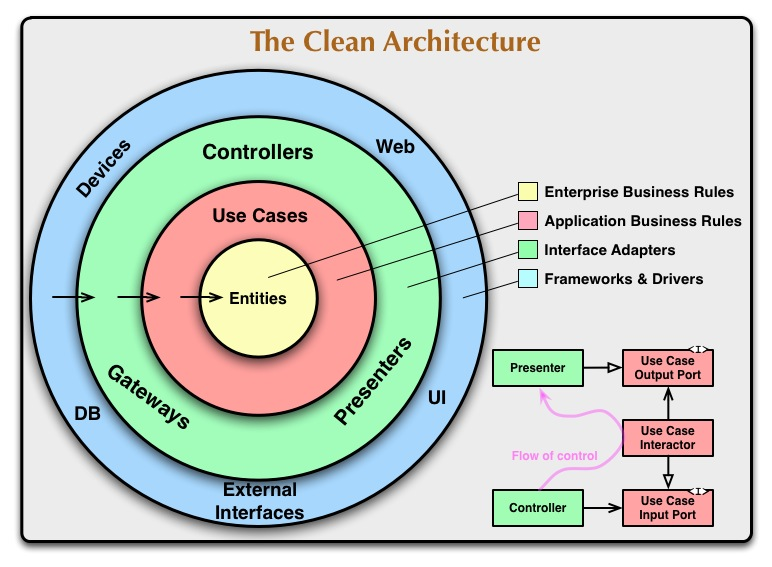
\includegraphics[width=0.9\linewidth]{figures/cleanarchitecture.jpg}
\caption{The clean architecture \cite[196]{martin2018clean}.}
\label{fig:cleanarchitecture}
\end{figure}

As seen in figure \ref{fig:cleanarchitecture}, this division results in four types of layers, guided by the various types of business rules and internal or external dependencies. This fragmentation of components facilitates the independent development, testing and evolution of the software layers. This philosophical perspective on software illustrates the importance of design in software, as system architecture can either motivate or inhibit developers from achieving their desired design goals.

%# History of programming languages and data formats
%% XML and its impact on JSON typesetting
%% Type-safe object-oriented programming
%% Extensibility in software development (language: Swift, data: [XML, TypeScript])

\pagebreak

The methodological approach...

% Grounded Theory as a methodological approach
%% Personas and other related design theory

\end{document}